\documentclass[10pt,twocolumn,letterpaper]{article}

\usepackage{cvpr}
\usepackage{times}
\usepackage{epsfig}
\usepackage{graphicx}
\usepackage{amsmath}
\usepackage{amssymb}
\usepackage[breaklinks=true,bookmarks=false]{hyperref}
\cvprfinalcopy
\graphicspath{ {./images/} }
\begin{document}

%%%%%%%%% TITLE
\title{\textsf{Advanced Algorithms project Report}}

\author{xxx xxx\\
University of Trento\\
Bachelor in Computer Science\\
{\tt\small xxx@studenti.unitn.it}
}

\maketitle
%\thispagestyle{empty}

\section{Introduction}

%-------------------------------------------------------------------------
The main objective of the project was to create an algorithm to identify, given an RGB image of a galaxy as input, the morphological class it belongs to. The morphological classes were 10 (\textit{Barred Spiral, Cigar Shaped Smooth, Disturbed, Edge-on with Bulge, Edge-on without Bulge, In-between Round Smooth, Merging, Round Smooth, Unbarred Loose Spiral, Unbarred Tight Spiral}). The dataset provided consisted of 17736 images, already divided in a training set and a test set. Ground truth labels were provided only for the train split. \\
Two metrics were used for evaluation, sample-wise accuracy ($Acc$) and class-wise accuracy ($mAcc$). In formulas:
\begin{center} 
$Acc =\frac{\text{\# correctly classified images}}{\text{\# of images}}$ 
\end{center}
\begin{center} 
$mAcc = \frac{1}{|\mathcal Y|}\sum_{y\in\mathcal Y} \frac{\text{\# of correctly classified images of class $y$}}{\text{\# of images of class $y$}}$
\end{center}

\section{Proposed Method}

I have considered both deep and shallow methods in order to better understand their strengths and limitations. For this specific problem classical algorithms, like \textit{Decision Tree}, \textit{K-Nearest Neighbors} and \textit{Support Vector Machine} are a bit complicated to use because we have a lot of images and pixels. 
They usually suffers of long training time or interference with large size inputs. Considering this I decided to opt for a more straightforward and powerful solution, I started by training a convolutional neural network. I used \textit{ResNet} which is one of the most popular modern networks. 

After I trained the neural network I was able to extract features by dropping the final layer. These features were then used to train and try traditional machine learning algorithms.

Since the test set was not labeled I had to split the training set in order to obtain a validation split. I used the \textit{train\_test\_split} function from the sklearn library\cite{scikit-learn} which also allows to split the set in a stratified fashion. I subsequently used the validation split to get an unbiased evaluation of the models performances, and to perform model selection (testing design choices, tuning hyper-parameters...).


\section{Results}

All approaches have been tried with different \textit{hyper-parameters} to improve performances.

\subsection{Neural Networks}

Every pre-trained model was taken from Pytorch website\cite{pytorch-models} and all features have been \textit{normalized}.

First of all I trained a Resnet50 without using any data augmentation technique. The dataset has been divided in mini-batches of size 64,
SGD was used as optimization function and Cross-Entropy was used as loss function. I then added a MultiStepLR scheduler. After some experiments I managed to find the best hyperparameters. 

To increase performances I have used some augmentation techniques on the training set. In particular I performed random vertical and horizontal flip, random rotation, and random crop using \textit{torchvision.transforms}\cite{torchvision-transforms}. Also, given that the dataset suffer of class imbalance, calculating class weights and using them as parameters in the Cross-Entropy Loss function has been useful to improve accuracy.

I decided to introduce checkpoints\cite{pytorch-checkpoints} for resuming training and since model’s performances on the validation set after the last epoch weren’t always the best.

Using ResNet50 the best result on the test set i managed to get was an $Acc$ of $0.840$ and a $mAcc$ of $0.808$.

I then decided to train ResNet152 in 30 epochs with the same hyper-parameters of ResNet50. I had to change the size of the mini-batches from 64 to 32 to fit the hardware memory. As you can see in the figure \ref{fig:resNet152}, using a model with more layers, I improved the results obtained previously.

\begin{figure}[h]
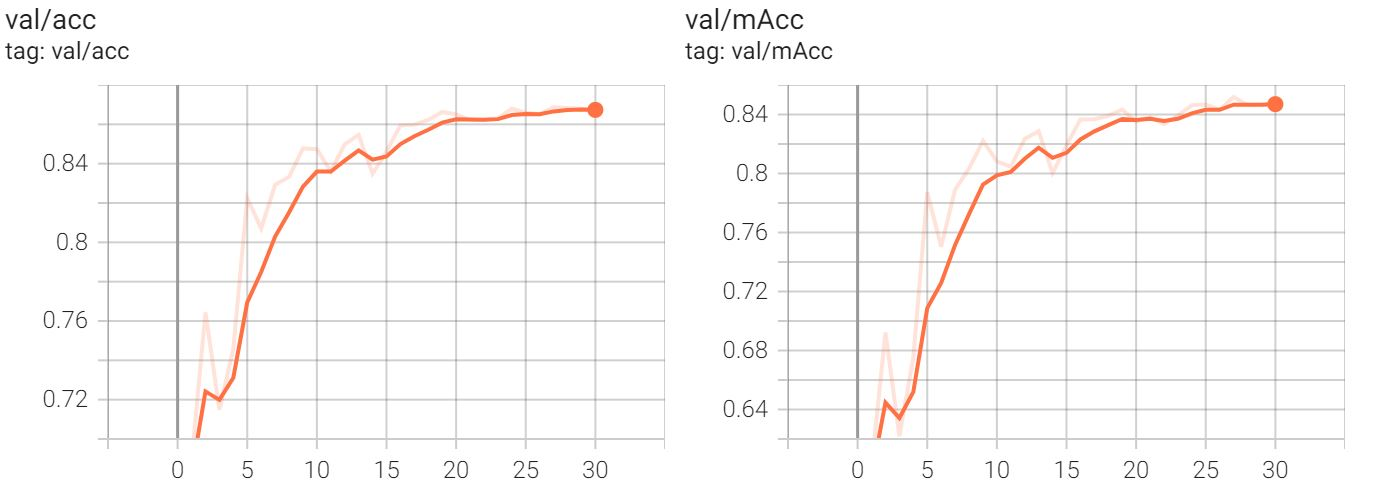
\includegraphics[width=\linewidth]{resnet152-val-acc}
\caption{ResNet152 validation performances}
\label{fig:resNet152}
\end{figure}

\noindent
However, it took much longer (10 minutes for each epoch) for training. 

On the test set I got an $Acc$ of $0.864$ and a $mAcc$ of $0.843$ using ResNet152. I believe these metrics could have been improved by training the model with even more epochs. 

\subsection{Traditional methods}

As I mentioned above, for testing traditional algorithms, the pre-trained ResNet152 has been used to extract features by dropping the final layer. This time the algorithms were taken from the scikit-learn library\cite{scikit-learn-sv-learning}.

\subsubsection{Decision Tree}

Different hyper-parameters have been tried with decision tree.
As show in the figure \ref{fig:DecisionTree} the best results ($Acc$ of 0.827 and a $mAcc$ of 0.808) were obtained using \textit{gini} as impurity measure together with \textit{25} samples for leaf. Using more samples for leaf has permitted to achieve a decent generalization. Performances were no better than those previously obtained with convolutional neural network.

\begin{figure}[h]
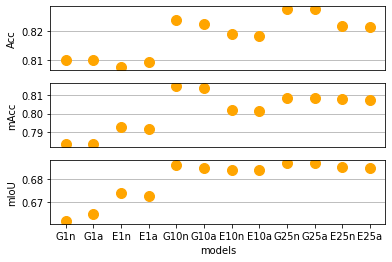
\includegraphics[width=\linewidth]{DecisionTree}
\caption{Decision trees performances on validation set}
\label{fig:DecisionTree}
\end{figure}

\subsubsection{K-Nearest Neighbors}

The K-Nearest Neighbors algorithm performed better than the decision tree, in fact using 11 as the number of neighbors (K) I obtained an $Acc$ of 0.866 and a $mAcc$ of 0.850 on the validation set.
K-NN performances, obtained using various K hyper-parameters, can bee seen in the figure \ref{fig:NearestNeighbor}.

\begin{figure}[h]
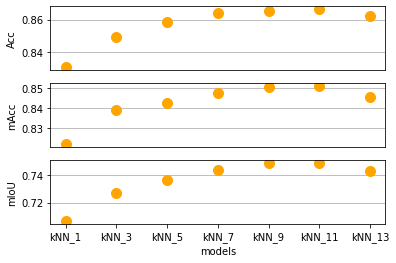
\includegraphics[width=\linewidth]{NearestNeighbor}
\caption{Nearest neighbor performances on validation set}
\label{fig:NearestNeighbor}
\end{figure}

\subsubsection{Support Vector Machine}

With SVM I tried radial-basis (R), linear (L) and polynomial (P) as kernel function, along with 0.1, 1, 10, 100 as regularization parameter C. The best result ($Acc$ of 0.872, $mAcc$ of 0.858 on validation set) was obtained using the radial-basis kernel function together with 10 as parameter C.

\begin{figure}[h]
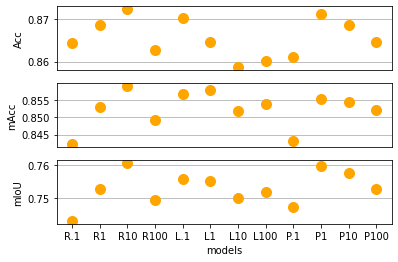
\includegraphics[width=\linewidth]{SVM}
\caption{SVM performances on validation set}
\label{fig:SVM}
\end{figure}

\subsection{Algorithms comparison}

In conclusion, the best performances were obtained by combining ResNet152 and SVM. To be specif the highest metrics on the test set were an $Acc$ of 0.871 and a $mAcc$ of 0.855.



{\small
\bibliographystyle{biblioStyle}
\bibliography{biblio}
}

\end{document}
